\documentclass[11pt,twoside]{article}
\usepackage{geometry}
\usepackage{enumerate}
\usepackage{latexsym,booktabs}
\usepackage{amsmath,amssymb}
\usepackage{graphicx}
\usepackage{hyperref}
\usepackage[singlespacing]{setspace}
\usepackage{calc}
\usepackage{blindtext}
\usepackage{subfig}
\usepackage{graphicx}

\geometry{a4paper,left=2cm,right=2.0cm, top=2cm, bottom=2.0cm}

\newtheorem{Definition}{Definition}
\newtheorem{Theorem}{Theorem}
\newtheorem{Lemma}{Lemma}
\newtheorem{Corollary}{Corollary}
\newtheorem{Proposition}{Proposition}
\newtheorem{Algorithm}{Algorithm}
\numberwithin{Theorem}{section}
\numberwithin{Definition}{section}
\numberwithin{Lemma}{section}
\numberwithin{Algorithm}{section}
\numberwithin{equation}{section}

\newcommand{\dottedline}[1]{\makebox[#1]{.\dotfill}}

\begin{document}

\pagestyle{empty}

% =============================================================================
% Title page
% =============================================================================
\begin{titlepage}
\vspace*{.5em}
\center
\textbf{\Large{The School of Mathematics}} \\
\vspace*{1em}
\begin{figure}[!h]
\centering

\includegraphics[width=180pt]{CentredLogoCMYK.jpg}
\end{figure}
\vspace{2em}
\textbf{\Huge{Anomaly Detection with Bayesian Neural Networks}}\\[2em]
\textbf{\LARGE{by}}\\
\vspace{2em}
\textbf{\LARGE{Theodoros Ladas}}\\
\vspace{6.5em}
\Large{Dissertation Presented for the Degree of\\
MSc in Statistics with Data Science}\\
\vspace{6.5em}
\Large{July 2021}\\
\vspace{3em}
\Large{Supervised by\\Dr Bruce Worton and Dr Daniel Paulin}
\vfill
\end{titlepage}

\cleardoublepage

% =============================================================================
% Executive summary, acknowledgments, and own work declaration
% =============================================================================
\begin{center}
\Large{Executive Summary}
\end{center}

Here comes your executive summary ...

\clearpage

\begin{center}
\Large{Acknowledgments}
\end{center}

Here come your acknowledgments ...

\clearpage

\begin{center}
\Large{University of Edinburgh – Own Work Declaration}
\end{center}


This sheet must be filled in, signed and dated - your work will not be marked unless this is done.
\vspace{1cm}

Name: \dottedline{8cm}

Matriculation Number: \dottedline{6cm}

Title of work: \dottedline{8cm}

\vspace{1cm}

I confirm that all this work is my own except where indicated, and that I have:
\begin{itemize}
\item	Clearly referenced/listed all sources as appropriate	 				
\item	Referenced and put in inverted commas all quoted text (from books, web, etc)	
\item	Given the sources of all pictures, data etc. that are not my own				
\item	Not made any use of the report(s) or essay(s) of any other student(s) either past 	
or present	
\item	Not sought or used the help of any external professional academic agencies for the work
\item	Acknowledged in appropriate places any help that I have received from others	(e.g. fellow students, technicians, statisticians, external sources)
\item	Complied with any other plagiarism criteria specified in the Course handbook
\end{itemize}

I understand that any false claim for this work will be penalised in accordance with
the University regulations	(\url{https://teaching.maths.ed.ac.uk/main/msc-students/msc-programmes/statistics/data-science/assessment/academic-misconduct}).								

\vspace{1cm}

Signature \dottedline{8cm}

\vspace{5mm}

Date \dottedline{8cm}


\clearpage



% =============================================================================
% Table of contents, tables, and pictures (if applicable)
% =============================================================================
\pagestyle{plain}
\setcounter{page}{1}
\pagenumbering{Roman}

\tableofcontents
\clearpage
\listoftables
\listoffigures
\cleardoublepage

\pagenumbering{arabic}
\setcounter{page}{1}

\nocite{*}
\bibliographystyle{abbrv}
\clearpage

% ------------------------------------------------------------------------------------------------------
\section{Introduction}

\subsection{Motivation}
\label{sec:motivation}
Anomaly detection is a very useful technique, leveraged (among others) by the banking sector in order to automaticaly block fraudulent transactions. This dissertation project is a detailed explanation of how an anomaly detection system could be implemented using Bayesian neural networks. This application, uses machine learning to train a model on a set of data, in order to predict an outcome of interest. Afterwards, the predictions are drawn many times (bootstraped), in order to create an estimation of confidence about the prediction. The goal of the project is to automatically flag transactions that could be fraudulent, thus allowing a human to spend time in deep investigation of those transactions, rather than manually going through each transaction one by one. 

This report is divided into the \textit{Introduction}, \textit{Exploratory Data Analysis}, \textit{Methods}, and \textit{Results} sections and a brief summary of each one is presented here. The rest of the \textit{Introduction} section will explain the specific dataset used for the presentation of the problem, as well as all the software requirements to be able to reproduce the results. Next, the \textit{Exploratory Data Analysis} section, presents a various aspects of the data, such as the distributions of the features, their corelations as well as a quick way to visually discover potential anomalies. On the \textit{Methods} section, the specific architecture of all the neural netwokrs models are presented, as well as the way the best model was selected (model validation). Finaly, three related but different metrics are presented in the \textit{Results} section of what constitutes as an anomaly, yet the specific threshhold for those metrics, is arbitrarily set. In a real life application this is a business decision, that should be set by the stakeholders according to their criteria. 

\subsection{Data Sources}
\label{sec:back}
The dataset used in this project, was given by the University of Edinburgh in the context of the dissertation project and it is the wine dataset. It is an especially clean and very well known real-life dataset for prototype creation. The basic assumption is that if the algorithm manages to capture anomalies on this dataset, it is in principal possible to productionise a variant of the architecture for an application of interest. More specifically it is a 4898 (rows) $\times$ 12 (columns) matrix, with no missing values and no duplicated rows. Each row represents one wine and the columns are the various features of each wine, such as its degrees of \textit{alcohol}, the \textit{acidity} of the wine, the \textit{pH} level wich measures how acidic or basic the solution etc. The problem this dissertation is going to try to solve, is a classification problem, of the \textit{type} of the wine, according to all other features. The variable \textit{type} is either \textit{1, 2, or 3} and the classes are almost perfectly balance thus making easier the preprocessing stage of the problem, and focusing more on the architecture and the interpretation of the algorithm as well as its results. Thus, the only preprocessing steps needed are the centering and scaling of the data matrix, to ensure that variables can potentially have the same impact regardless of the scale they are measured in and one-hot encoding the \textit{quality} feature, since its also not a numeric variable, but a factor one. Lastly, The dataset is split into train ($80\%$), validation ($25\%$) and test ($25\%$) sets to ensure that no algorithm overfits the given dataset. 

\subsection{Software}
\label{sec:software}
A combination of the programming languages \textsf{R} and \textsf{Python} are used to produce this report. The use of both languages is in no way binding. \textsf{R} is used for the exploration of the dataset, as well as for the dimensionality reduction plots, while \textsf{Python} is used in combination with \textsf{tensorflow},\textsf{tensorflow-probability}, and \textsf{keras} to build, validate, and test the neural networks. These packages can also be used from the \textsf{R} ecosystem, yet the setup process is more complicated and thus avoided. The reason \textsf{R} is selected for the EDA, is due to the \textsf{ggplot2} package, wich is a very powerfull and easy package for creating complicated plots.
\clearpage


%------------------------------------------------------------------------------------------------------
\section{Exploratory Data Analysis}
In this section a basic overview of the dataset and its properties is going to be presented. Firstly, various statistics regarding the dataset are presented in the form of graphs, in univariate, bivariate and multivariate analysis. Afterwards, the dataset it reduced in dimensions with two techniques (a linear and a non-linear) in order to be able to plot it with a two-dimensional graph. This is also a quick way to identify potential anomalies as well visually. The reason of the extended EDA, is to understand what preprocessing steps could be needed in order for the future models to work correctly. Also, the knowledge gained from this exploration of the dataset will help in the explanation of the model in the \textit{Model Validation} section. 

\subsection{Univatiate Analysis}
\label{sec:univariate}
The dataset, consist of twelve feature variables, out of which only one (\textit{quality}) is categorical, while all the others are numeric. The target varaiable (\textit{type}) is also a target variable with three levels \textsf{type=1, type=2, type=3}. There are no missing values.

\vspace*{1em}
\begin{figure}[!h]
\centering
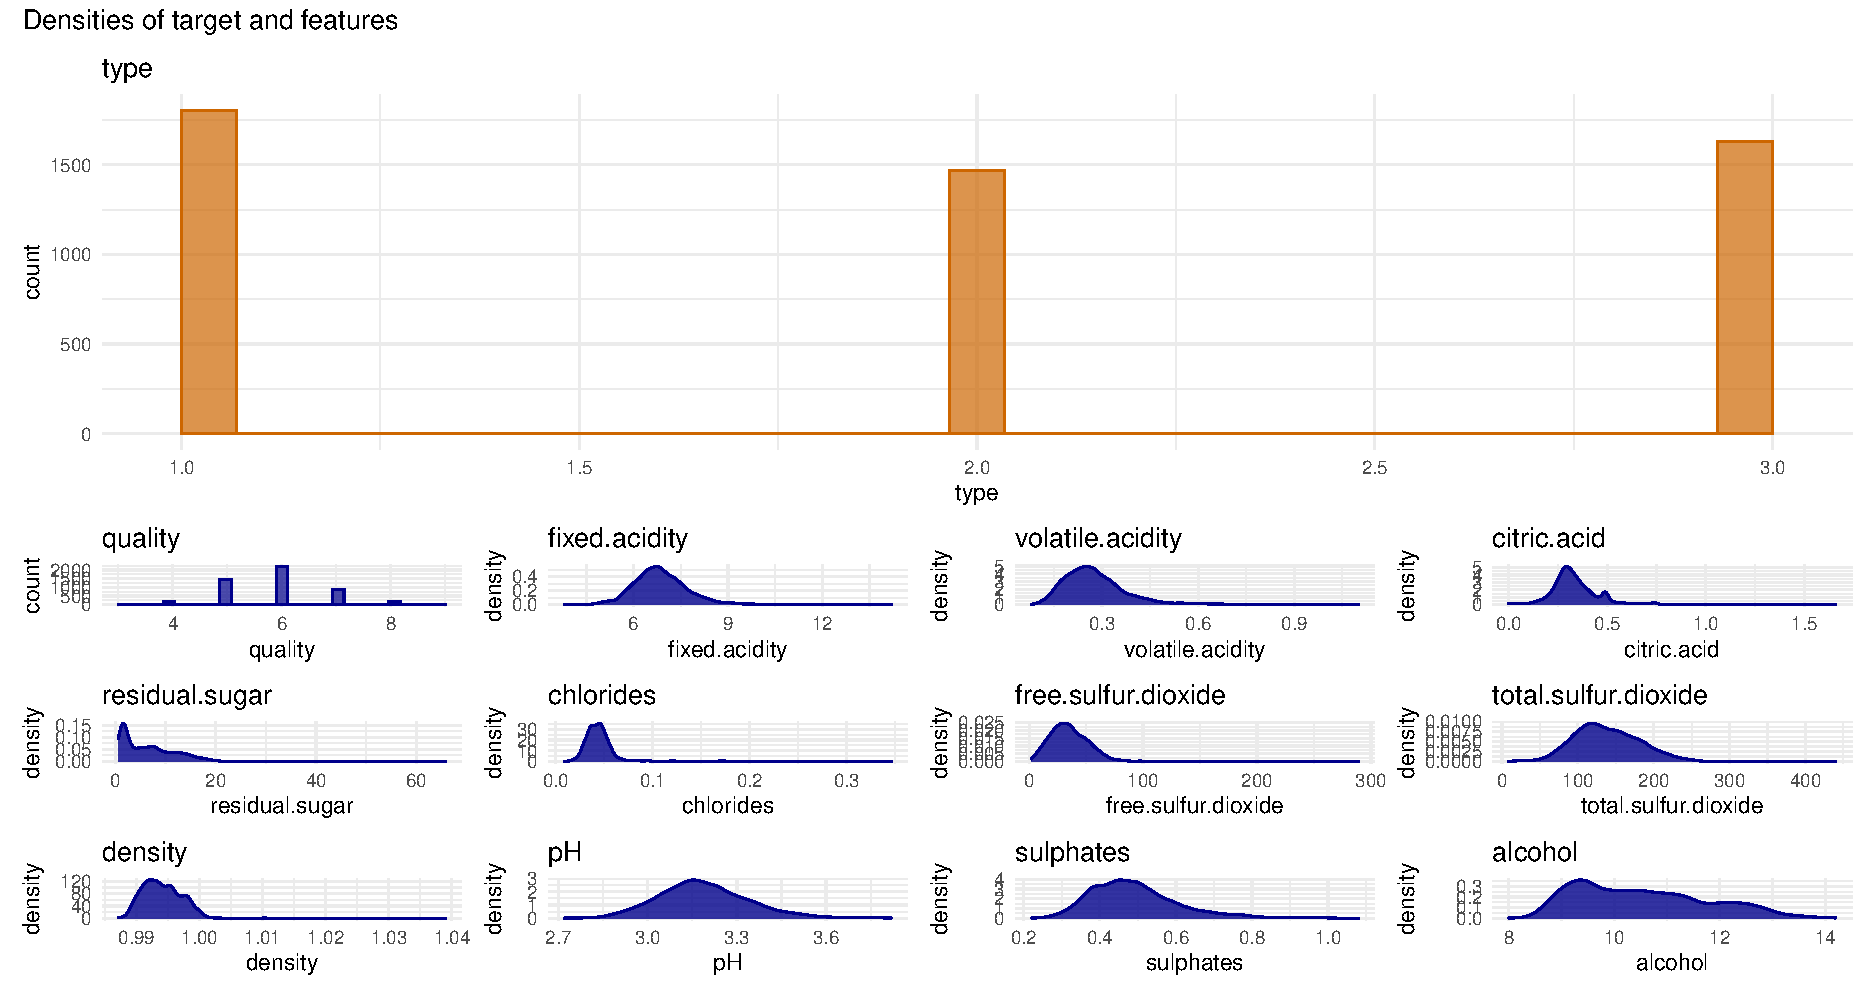
\includegraphics[width=\textwidth]{./output/1.h.univariate-analysis.pdf}
\caption{centered image}
\label{fig:uni}
\end{figure}
\vspace{2em}

In \autoref{fig:uni}, the target variable type is represented by the orange barplot. The number of rows in each class is balanced therefore no preprocessing to upsample (downsample) the underepresented (overrepresented) classes is needed. On the variable \textit{quality}, the majority of cases are \\
 $(quality\geq5) \lor (quality\leq7)$, which would make the very poor and very good wines difficult to predict. Finally, evidently the features, are measured in vastly different scales. For example \textit{pH} is ranging from 2.7 to 3.6, while \textit{free.residual.dioxide} is ranging from 0 to 300. This means that centering and scaling the data matrix is crusial for any algorithm to work properly.

\subsection{Bivariate Analysis}
\label{sec:bivariate}

Extending the univariate analysis of the previous subsection, the bivariate analysis reveals how the feature correlate to each other. \autoref{fig:corr} (a) and \autoref{fig:corr} (b) are both producing the same information but presented differently. On \autoref{fig:corr} (a) the exact values of the linear relationships are shown, while on \autoref{fig:corr} (b) clear clusters of high and low linear correlation are formed. Out of these clusters that are present in \autoref{fig:corr} (b) some are expected but others are not.

For measuring the correaltion, the \textit{Pearson's correlation coefficient} is used, which measures the covariance of two random variables, $X$ and $Y$, and normalizes it with the product of their standard deviations, or:

\begin{equation}
\rho(x,y) = \frac{\text{cov}(x,y)}{\text{std}(x)\text{std}(y)}
\end{equation}

\begin{figure}[h]
    \centering
    \subfloat[Recipe length distribution with KDE]
    {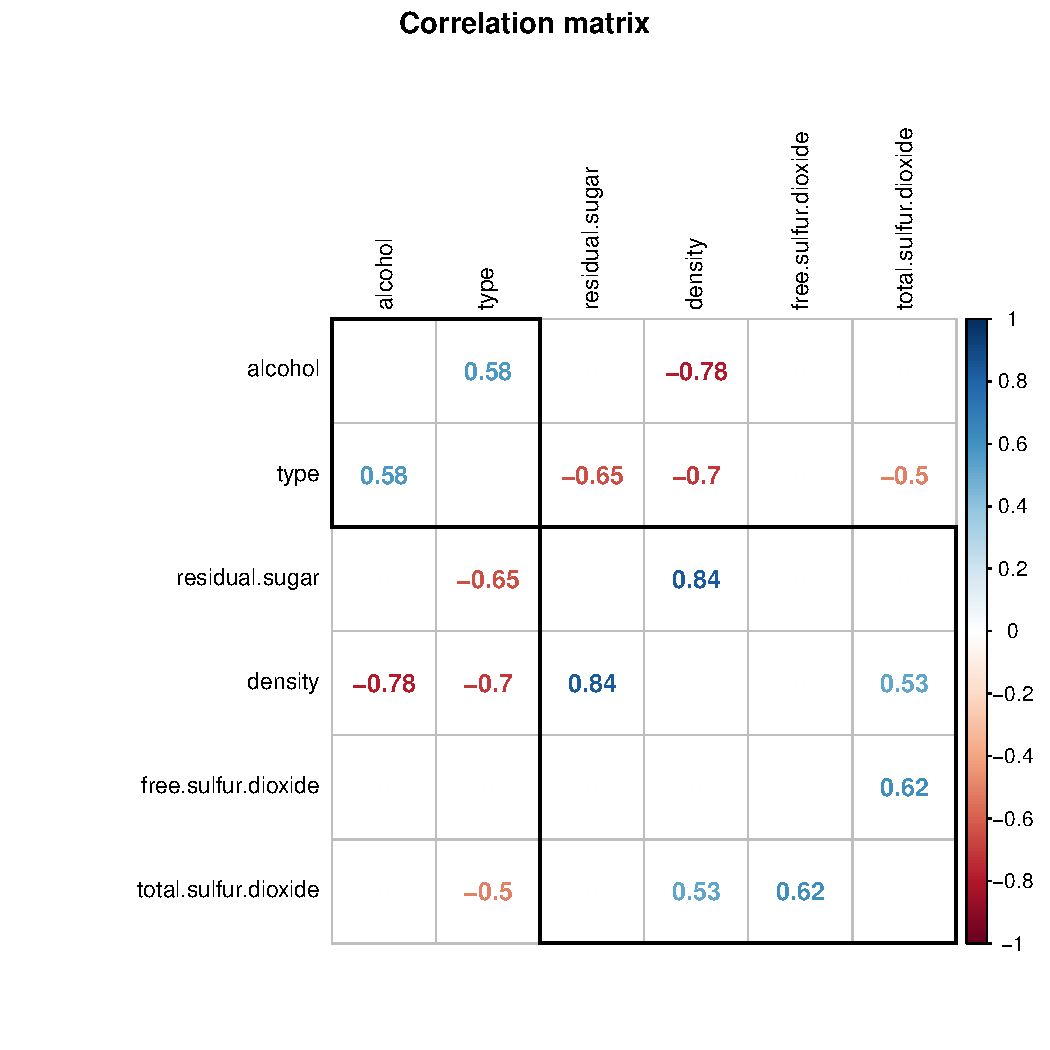
\includegraphics[width=.4\textwidth,height=.25\textheight]{./output/1.e.corrplot-1.pdf}}
    \subfloat[Top 20 Ingredients]
    {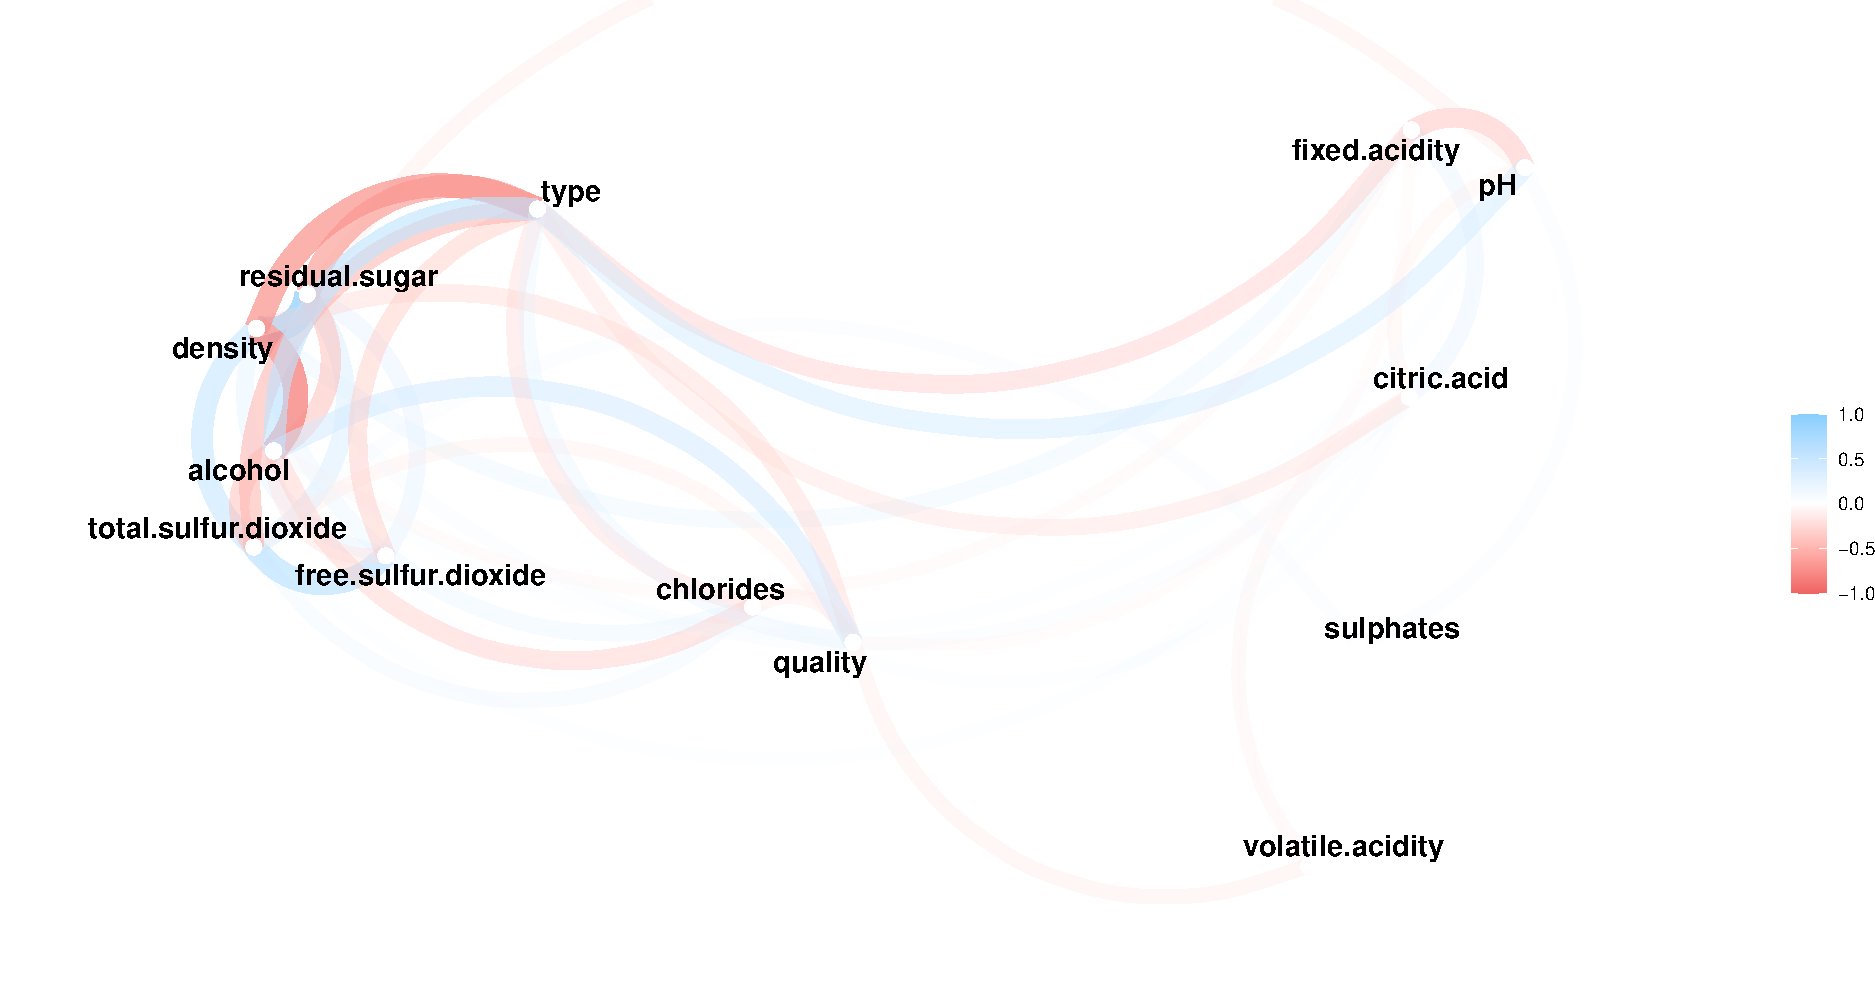
\includegraphics[width=.6\textwidth]{./output/1.f.corplot-2.pdf}}
    \caption{}
    \label{fig:corr}
\end{figure}

For example, \autoref{fig:corr} (a) shows a strong positive relationship between \textit{free.sulfur.dioxide} and \textit{total.sulfur.dioxide}, which is expected, as \textit{total.sulfur.dioxide} is the \textit{free.sulfur.dioxide} plus other sulfur dioxides from other ingredients. Intrestingly, the same is not true regarding \textit{volatile.acidity}, \textit{fixed.acidity} and \textit{citric.acid}. The feature with the most strong correlations however, is \textit{density}, as it strongly correlates, both positively or negatively with \textit{alcohol}, \textit{type}, \textit{residual.sugar} and \textit{total.sulfur.dioxide}. 

In general we identify two clusters. One with strong correlations containing \textit{type}, \textit{residual.sugar}, \textit{density}, \textit{alcohol}, \textit{total.sulfure.dioxide} and \textit{free.sulfure.dioxide}, and a second one with low correlations containing \textit{fixed.acidity}, \textit{pH}, \textit{citric.acid}, \textit{sulphates} and \textit{volatile.acidity}. The model is going to leverage this relationships in order to predict the outcome. 

\subsection{Dimensionality Reduction}
\label{sec:reduction}
In the exploration of the dataset, two different techniques were used in order to reduce the dimensions and visualize it with plots. The first method is the Principal Component Analysis (PCA), which a singular value decomposition (SVD) of the centered, data matrix. The SVD of an $ m \times n $ matrix $A$ is the factorization of the matrix into $USV^\top$. Secondly, a more advanced nonlinear dimensionality reduction method, called t-distributed Stochastic Neighbor Embedding (t-SNE) was tryied, to cross evaluate the results of PCA. This methods works by finding a way to project the high dimensional data into a lower dimension, while preserving the culstering of the higher dimension.

\subsubsection{PCA}
\label{sec:pca}

Using the singular value decomposition to factorize the data matrix $X$, we produce, three matrixes, $U$, $S$ and $V$, each carrying information about the dataset in some aspect. First of all, we can create the following graph of the percentage of variance explained by each principal component. 
%----------
\vspace*{1em}
\begin{figure}[!h]
\centering
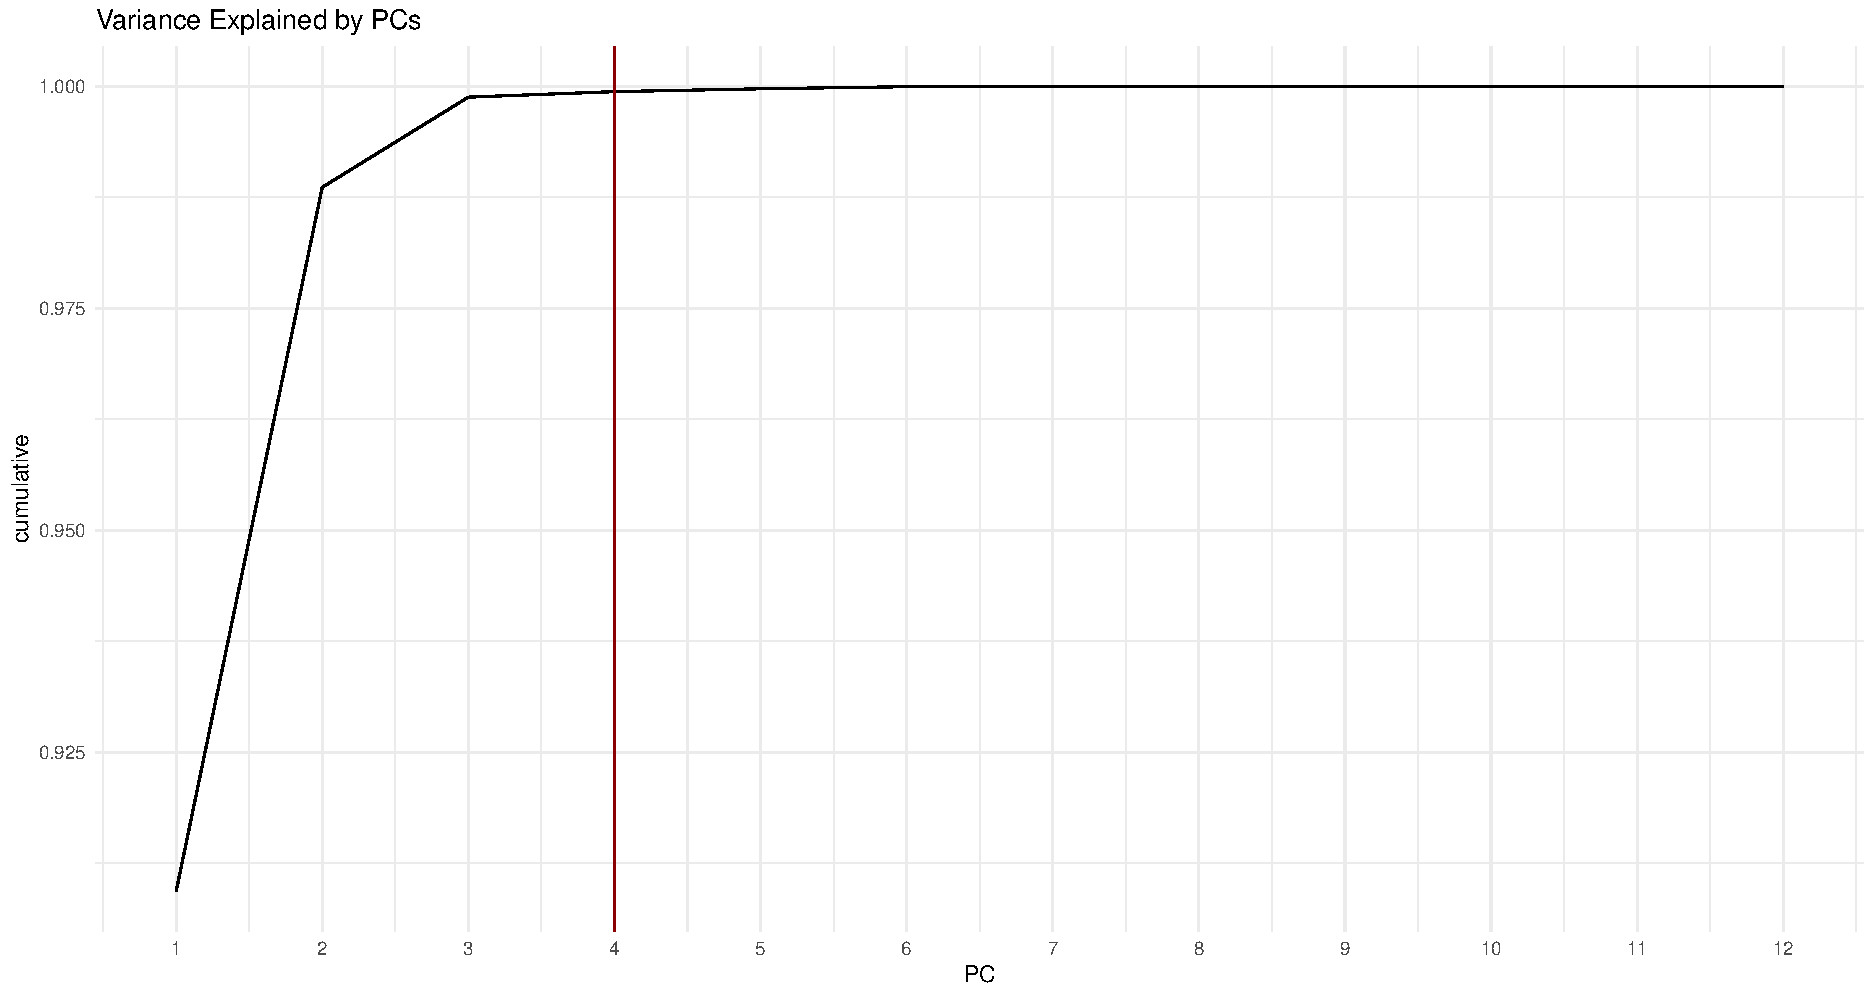
\includegraphics[width=\textwidth]{./output/1.a.pca-var-expl.pdf}
\caption{}
\label{fig:var_expl}
\end{figure}
\vspace{2em}
%----------

In \autoref{fig:var_expl}, we can see the cummalative variance explained by each additional principal component. This is a very important graph as we can reduce the dimension of the data matrix by selecting a threshold (for example, 99\% of the variance). In this example, it is clear that with only the first four principal components, that threshold is surpassed.

The principal components are a linear compination of all the columns of the dataset, and each one is perpandicular to the previous one. We can continue the exploration by visualizing the weights (loadings) of these four principal components and try to understand wheather these components make sense according to our knowledge on the topic. 

%----------
\vspace*{1em}
\begin{figure}[!h]
\centering
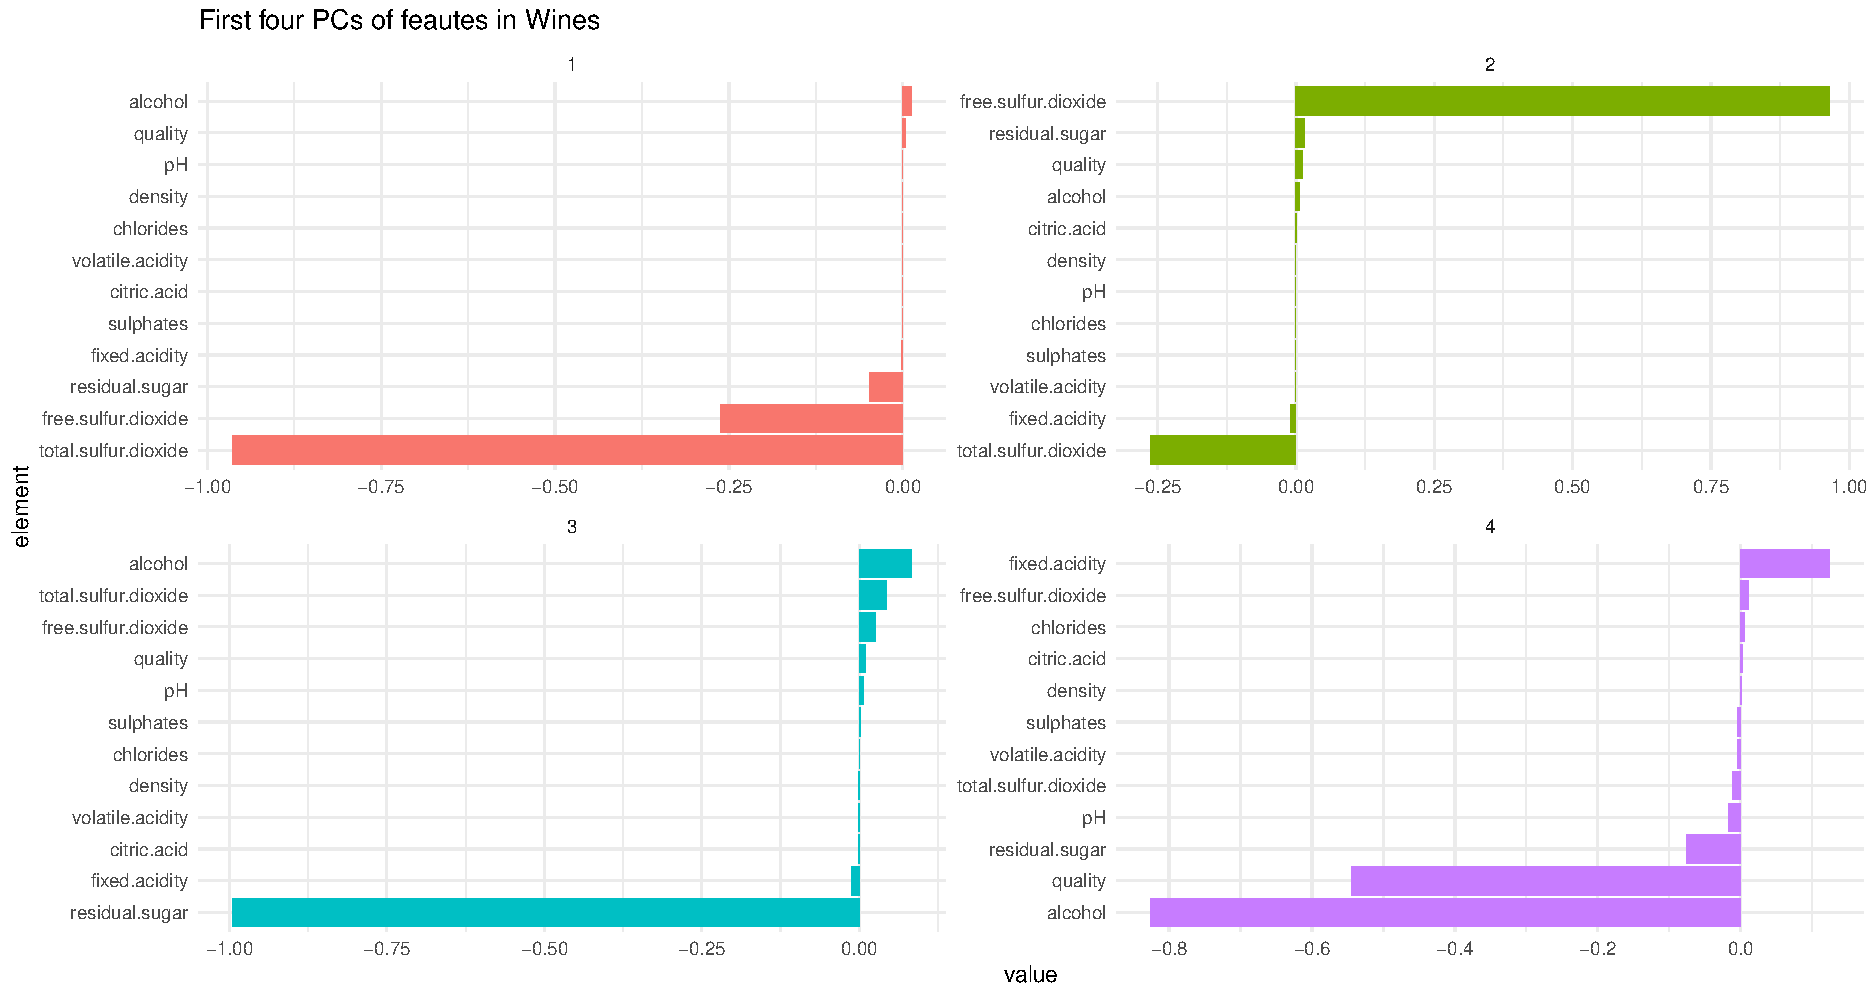
\includegraphics[width=\textwidth]{./output/1.b.pca-features.pdf}
\caption{centered image}
\end{figure}
\label{fig:pca_f}
\vspace{2em}
%----------

In \autoref{pca_f} the first four principal components are visualized along with the loadings of each columns. By on the two most extreme positive and negative values of the loadings, we can interpret the components into new kinds of variables. 

\begin{itemize}
\item PC1: Alcohol vs Sulfur Dioxide (free and total)
\item PC2: Free Sulfur Dioxide vs Total Sulfur Dioxide
\item PC3: Alcohol vs Sugar
\item PC4: Alcohol vs Acidity
\end{itemize}

It is clear that this dimensionality reduction technique produces results that reflect the real word. Sulfure Dioxide is a vital component in wine making as it regulates bacteria growth among other important tasks, yet, it also gives unpleasent oddors and tastes to the wine. PCA immidiately captures that reality by assigning the two biggest negative loadings on sulfure dioxide concentration (both free and total) to the first pricnipal component. In addition to that, the second most important component in order to classify the wines, is the origin of that Sulfure Dioxide. The total Sulfure Dioxide is the Free Sulfure Dioxide plus Sulfure Dioxide that is bound to other ingredients such as sugars etc. After investigating how much SO2 a wine has, as well as were it comes from (free vs total), the next most important factors have to do with the specific taste of the wine, mainly how sweet and how acidic the taste the wine has. 

We can now visualize the first two pricnipal components on a plot, while also coloring the datapoint according to their \textit{type}, the target variable. 
%----------
\vspace*{1em}
\begin{figure}[!h]
\centering
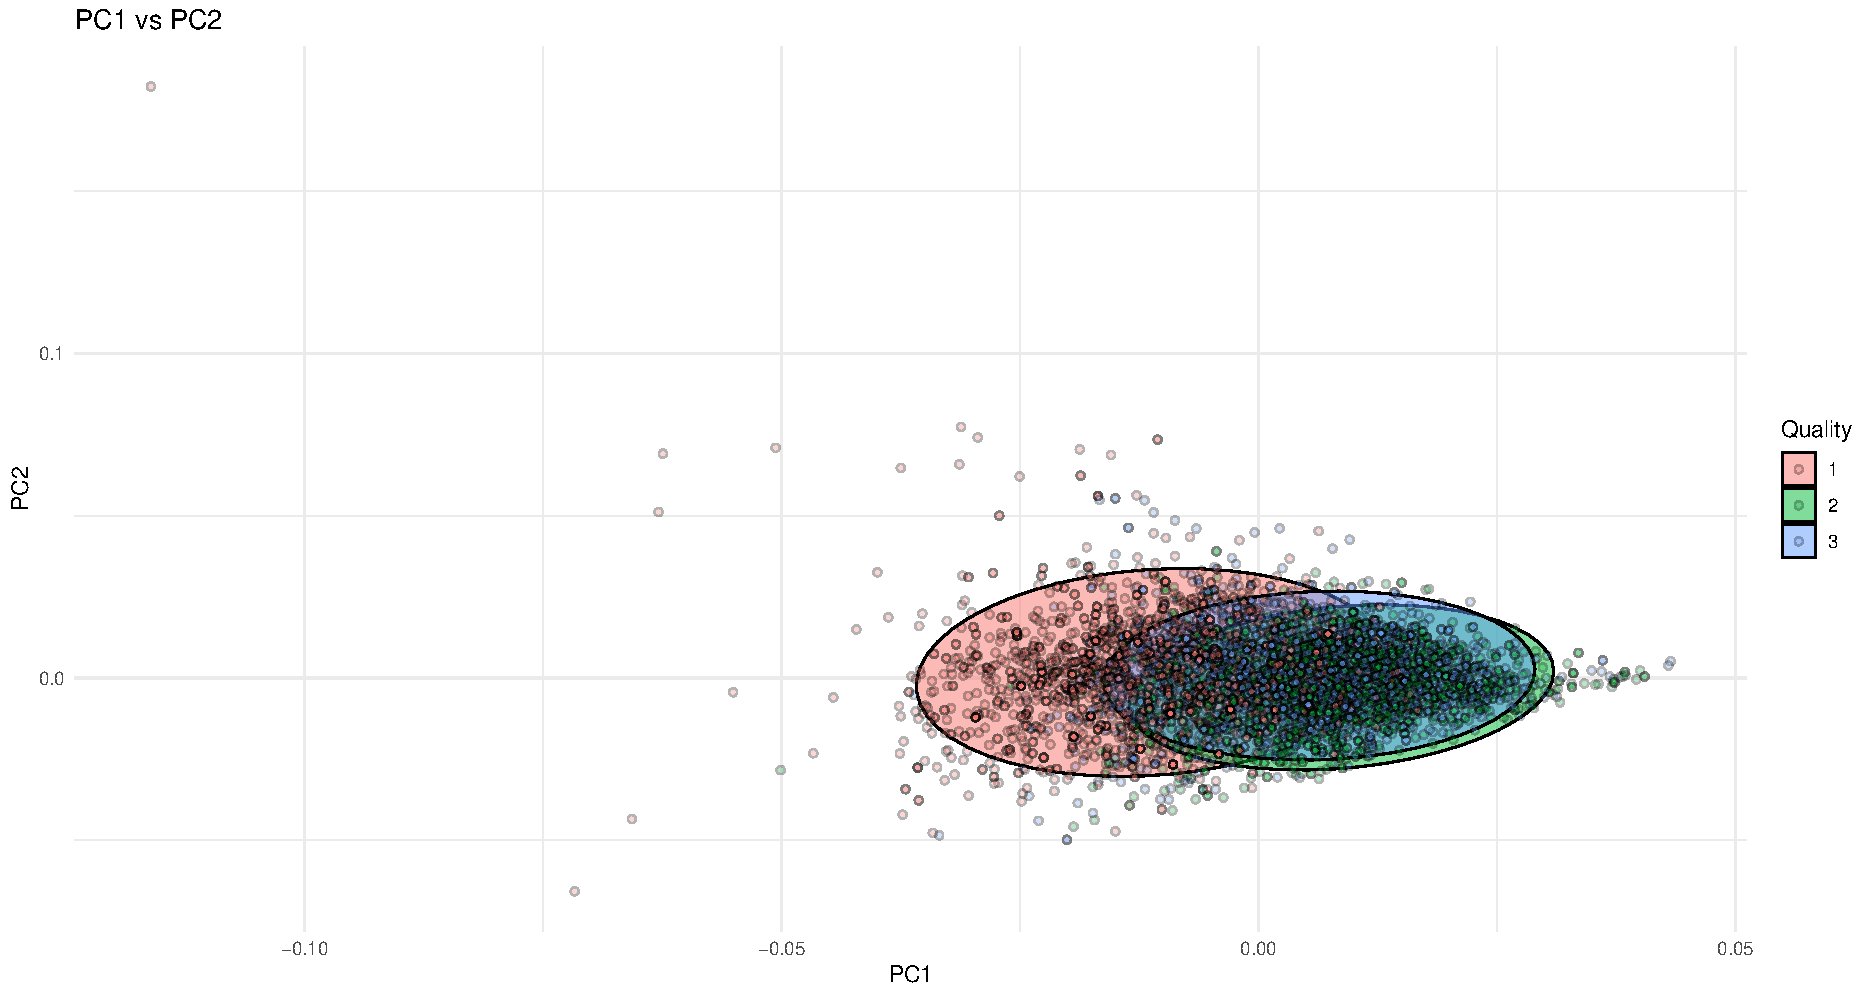
\includegraphics[width=\textwidth]{./output/1.c.pca-biplot.pdf}
\caption{centered image}
\label{fig:pca_biplot}
\end{figure}
\vspace{2em}
%----------
It is immidiately clear by \autoref{fig:pca_biplot} that \textit{type} classes two and three, have an extensive overlap in this graph. That is a useful information in the model evaluation, as we expect the model to "find it difficult" to distinguish a wine of type two from a wine of type three, while simultaneously having better accuracy in predicing class one. However, there a second major takeaway from \textit{Figure 3}, and that is the existance of potential anomalies. While the majority of the points are centered around $(0,0)$, some points are geometrically far away from the others of the same class. 

\subsubsection{t-SNE}
\label{sec:tsne}

Princiapal Component Analysis through singular value decomposition produced important findings and deepened our undestanding of the dataset. However, it was clear by \textit{Figure 3}, that it could not produce a clear enough separation between the classes. This could be because of the nature of the dataset, or it means that PCA is too simple to capture the complexity of the dataset, due to its linear nature. 

Therefore, a second, non-linear technique was tried in order to produce the corresponding figure as \textit{Figure 3}. This technique, is based on calculating the distances from each point to each neighbords and imposing a t-distribution on those values. It is an iterative algorithms that many times produces very good clustering.  However, in \autoref{fig:sne_biplot}, it is clear that \textit{type} classes two and three are still clustered together, while class one, is separated. 

The main takeaway from this analysis is that the dataset, although clean and simple in nature to understand, is mode complicated than it looks. This suggest that a simple model such as logistic regression might not be the model of choice. Neural Networks are a good candiate for such task due to their flexible nature. 

%----------
\vspace*{1em}
\begin{figure}[!h]
\centering
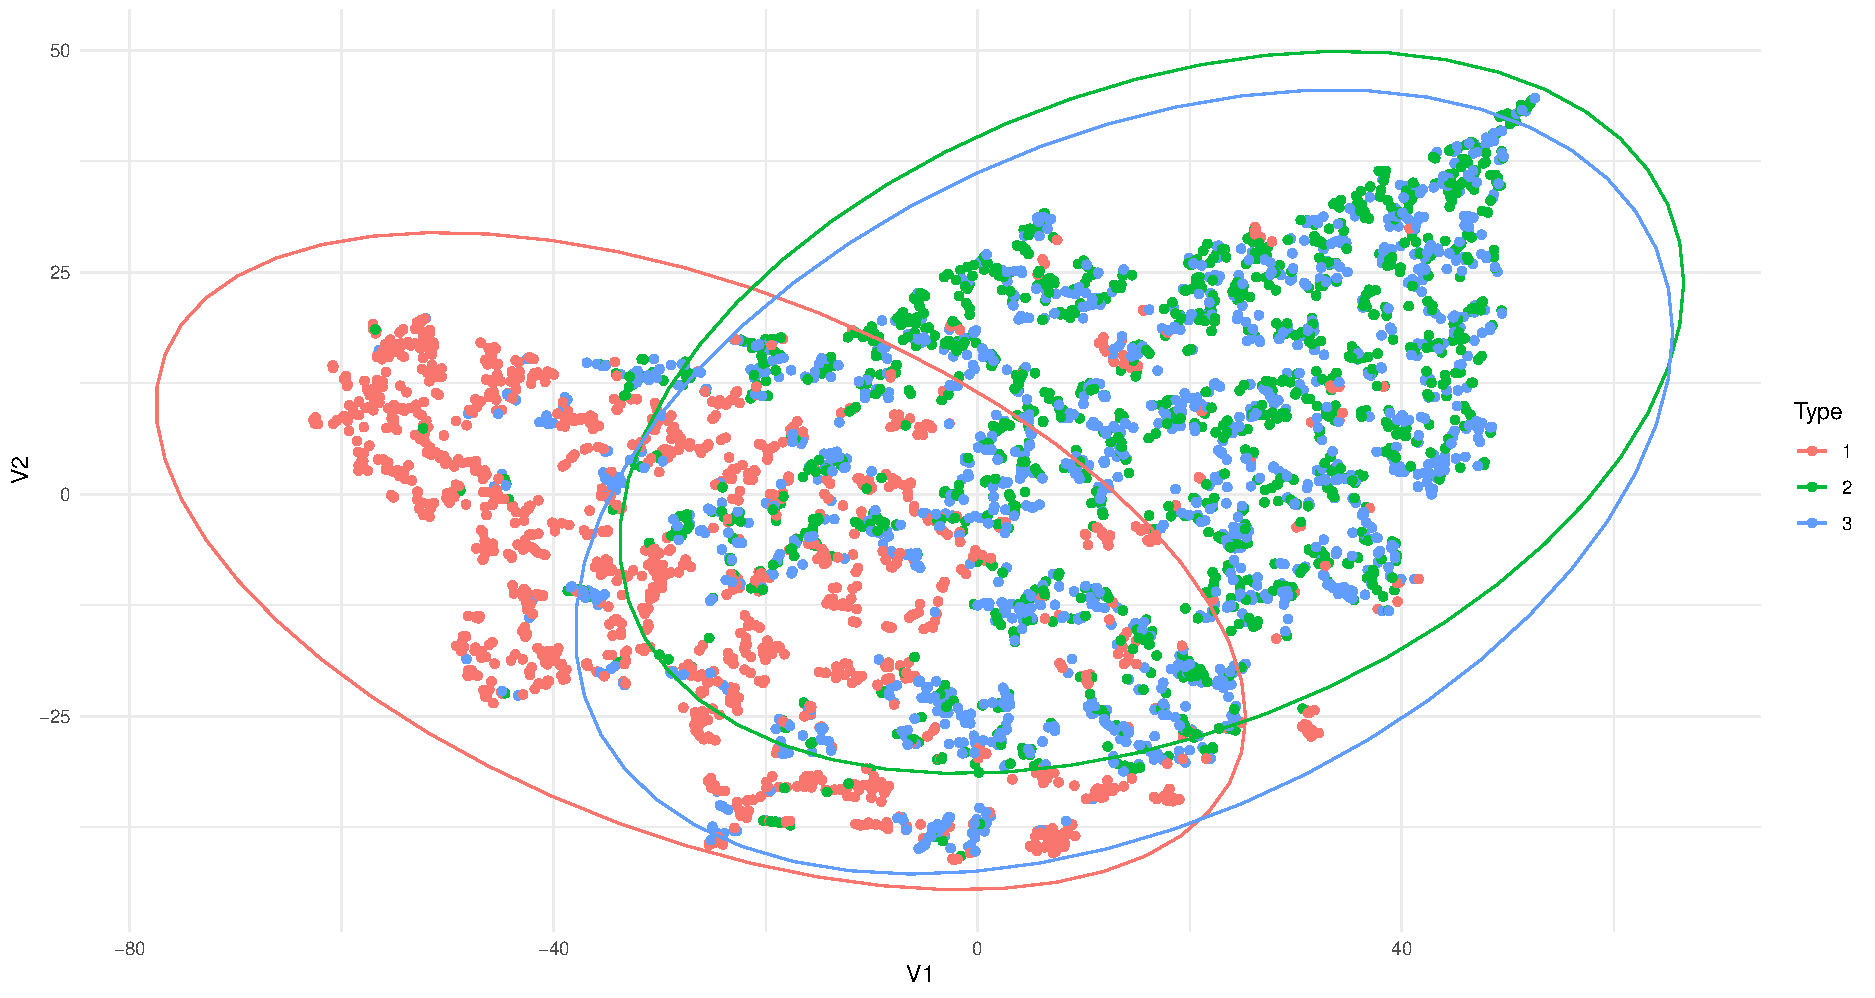
\includegraphics[width=\textwidth]{./output/1.d.t-sne.pdf}
\caption{centered image}
\label{fig:sne_biplot}
\end{figure}
\vspace{2em}
%----------


\subsection{Multivariate Analysis}
\label{sec:multivariate}
\blindtext


\clearpage


% ------------------------------------------------------------------------------------------------------
\section{Methods}
\label{sec:methods}
\blindtext

\subsection{Base Neural Network}
\label{sec:NN}
\blindtext

\subsection{Bayesian Neural Network}
\label{sec:BNN}
\blindtext


\subsection{Model Validation}
\label{sec:validation}
\blindtext

\subsection{Model Explanation}
\label{sec:explanation}
\blindtext

\clearpage

% ------------------------------------------------------------------------------------------------------
\section{Results}
\label{sec:results}
\blindtext

\subsection{Standard Deviation}
\blindtext

\subsection{Confidence Intervals}
\blindtext

\subsection{Entropy}
\begin{figure}[!ht]
\centering
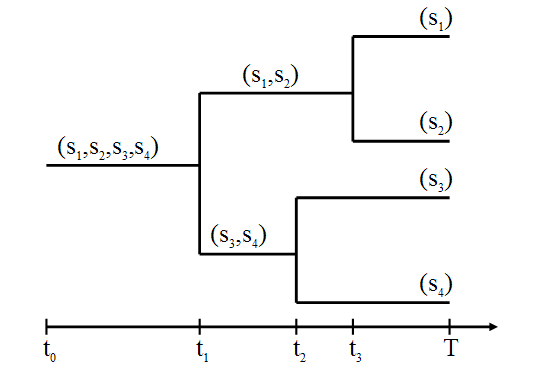
\includegraphics[width=8cm]{scenTree.png}
\caption{Look at this scenario tree with funny times $t_{1}$ and scenarios $s_{1}$ etc.}
\label{fig:scenarioTree}
\end{figure}

\cleardoublepage

% ------------------------------------------------------------------------------------------------------
\section{Discussion}
\blindtext
\clearpage

% ------------------------------------------------------------------------------------------------------
%tliterature.bib
\bibliography{literature}
\clearpage

% ------------------------------------------------------------------------------------------------------
\appendix
\section*{Appendices}
\addcontentsline{toc}{section}{Appendices}
\blindtext

\section{Appendix first topic}
\label{app:one}
\blindtext

\section{Appendix second topic}
\label{app:one}
\blindtext
\clearpage

\end{document}
